\chapter{Phương pháp dựa trên luật}
\label{chap:RuleBase}

Trong phần này chúng tôi mô tả lại cách mô hình hóa lại bài toán theo phương pháp dựa trên luật AnyBURL,thuật toán lấy mẫu luật (đường đẫn) và thuật toán khái quát hóa một luật để lưu trữ trở thành tri thức của mô hình. Cùng với những cải tiến của chúng tôi trong quá trình đào tạo khi có một tri thức mới được thêm vào đồ thị(thêm cạnh).

\section{Luật Horn}
Trong logic toán học, một công thức nguyên tử (\textbf{atomic formula})\cite{wiki:Atomic} còn được gọi đơn giản là một (nguyên tử-\textbf{atom}) là một công thức không có cấu trúc mệnh đề, nghĩa là một công thức không chứa các liên kết logic (\(\vee, ~ \wedge\)) hoặc tương đương (\(\Leftrightarrow\)) là một công thức không có các mẫu con nghiêm ngặt (tức là atom không thể chia nhỏ ra thành các atom con nữa). Do đó, các công thức nguyên tử là công thức đơn giản nhất để hình thành luật của logic. Các công thức hợp được hình thành bằng cách kết hợp các công thức nguyên tử bằng cách sử dụng các liên kết logic.

Một \textbf{literal}\cite{wiki:Literal} là một công thức nguyên tử (atom) hoặc phủ định của nó. Định nghĩa chủ yếu xuất hiện trong lý thuyết logic cổ điển. \textbf{Literal} có thể được chia thành hai loại: Một \textbf{positive literal} chỉ là một nguyên tử (ví dụ: \(x\)). Một \textbf{negative literal} là phủ định của một nguyên tử (ví dụ: \(\neg x\)). Sự phân chia của \textbf{literal} là \textbf{positive literal} hay \textbf{negative literal} tùy thuộc vào việc \textbf{literal} được định nghĩa.

Một mệnh đề (clause) là một literal hoặc nối rời của hai hoặc nhiều literal. Ở dạng \textbf{Horn} một mệnh đề có nhiều nhất một positive literal. Lưu ý: Không phải mọi công thức trong logic mệnh đề đều có thể đưa về dạng Horn.Mệnh đề xác định không có literal đôi khi được gọi là mệnh đề đơn vị (unit clause) và một mệnh đề đơn vị không có biến đôi khi được gọi là \textit{facts}\cite{wiki:Horn}.Một công thức nguyên tử được gọi là \textit{ground} hoặc \textit{ground atoms} nếu nó được xây dựng hoàn toàn từ các mệnh đề đơn vị; tất cả các \textit{ground atoms} có thể ghép lại từ một tập hợp hàm và các ký hiệu vị từ nhất định tạo nên cơ sở Herbrand cho các bộ ký hiệu này\cite{wiki:Term}.

\section{Định nghĩa ngôn ngữ đồ thị  tri thức} \label{kg}

Khác với các định nghĩa về đồ thị tri thức tổng quát được đùng cho các phương pháp nhúng đồ thị. Trong phương pháp dựa trên luật của chúng tôi. Chúng tôi xem đồ thị như là một ngôn ngữ hình thức. Dưới đây là các định nghĩa theo ngôn ngữ hình thức của đồ thị tri thức.

Một đồ thị tri thức \(\mathbb{G}\) được định nghĩa trên một bộ từ vựng \(\langle \mathbb{C}, \mathbb{R} \rangle\) trong đó \(\mathbb{C}\) là tập hợp các hằng số và \(\mathbb{R}\) là tập hợp các vị từ nhị phân.Khi đó, \(\mathbb{G} = \{r (a, b) \mid r \in \mathbb{R}, a, b \in \mathbb{C}\}\) là tập hợp các \textit{ground atoms} hoặc \textit{facts}. Một vị từ nhị phân được gọi là quan hệ và hằng số (hoặc hằng số được đề cập đến) được gọi là thực thể (entity) tương ứng với một dòng dữ liệu trong tập huấn luyện. Sau đây chúng tôi sử dụng các chữ cái viết thường cho các hằng và chữ in hoa cho các biến cho các thảo luận dưới đây. Vì chúng ta không học các quy tắc Horn tùy ý, và chỉ học đối với loại quy tắc nào có thể được khái quát hóa như được thảo luận dưới đây.

Chúng ta định nghĩa một quy tắc là \(h(c_0, c_n) \gets b_1(c_0, c_1) ,\dots ,b_n(c_{n}, c_{n + 1})\) là một đường dẫn ground atoms có chiều dài \(n\). Trong đó \(h(\dots)\) được gọi là \textit{head atoms} và \( b_1(c_0, c_1) ,\dots ,b_n(c_{n}, c_{n + 1})\) được gọi là \textit{body atoms}. Chúng tôi sẽ phân biệt dưới đây ba loại quy tắc mà chúng tôi gọi là: \textit{quy tắc nhị phân} \((\mathbf{B})\) là quy tắc trong head atoms chứa 2 biến, quy tắc đơn nguyên kết thúc bằng một đỉnh treo  và atom này chỉ chứa biến không chứa hằng số\((\mathbf{U_d})\) và head atoms chỉ chứa 1 biến. Còn quy tắc đơn nguyên kết thúc bằng một atom \((\mathbf{U_c)}\) và head atoms cũng chỉ chứa 1 biến.\((\mathbf{U_c)}\)  có thể là một đỉnh treo tới một hằng số bất kì nếu hằng số này trùng mới hằng số trong head atom thì tạo thành một đường đẫn có chu trình.

\[B \hspace{3.7cm} h(A_0,A_n) \gets  \bigwedge^n_{i=1} b_i(A_{i-1}, A_i)\]
\[U_d \hspace{3.8cm} h(A_0,c) \gets  \bigwedge^n_{i=1} b_i(A_{i-1}, A_i)\]
\[U_c \hspace{1cm} h(A_0,c) \gets  \bigwedge^{n-1}_{i=1} b_i(A_{i-1}, A_i) \wedge b_n(A_{n-1}, c^{\prime})\]

Chúng tôi gọi các quy tắc của các loại này là quy tắc đường đi (path rules), bởi vì các body atoms (phần sau đấu \(\gets\)) tạo thành một đường đi. Lưu ý rằng nó cũng bao gồm các biến thể quy tắc với các biến được đảo ngược trong các nguyên tử: được đưa ra trong đồ thị tri thức \(\mathbb{G}\), đường dẫn có độ dài \(n\) là một chuỗi gồm \(n\) bộ ba \(p_i (c_i, c_i + 1)\) với \(p_i (c_i, c_i + 1) \in \mathbb{G}\) hoặc \(p_i (c_i + 1, c_i) \in \mathbb{G}\) với \(0 \geq i \leq n\). Các mẫu quy tắc trừu tượng (abstract rule patterns) được cho ở trên có độ dài \(n\) vì body atoms của chúng có thể được khởi tạo thành một đường dẫn có độ dài \(n - 1\). Ví dụ như \hyperref[fig:burl]{hình 3.1}. Khi lấy mẫy đường đãn với độ dài bằng 3 chúng ta có thể có hai quy tắc sau: Quy tắc được đánh đấu màu xanh lá cây và quy tắc được đánh dấu màu đỏ 
\[speaks(ed, d) \gets married(ed, lisa) \wedge born(lisa, a) ~~~ \text{(xanh lá cây)}\]
\[\hspace{0.7cm}speaks(ed, d) \gets lives(ed, nl) \wedge lang(nl, d) ~~~ \text{(đỏ)} \]

\begin{figure*}[htp]
	\centering
	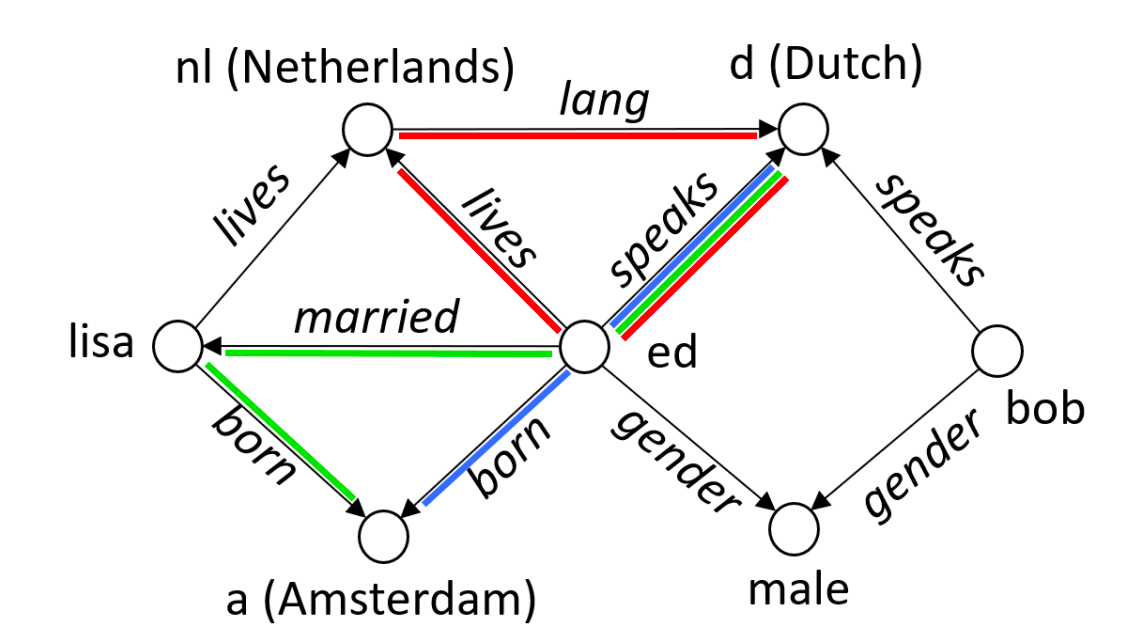
\includegraphics[width=12cm]{burl-ago.png}
	\caption{Ví dụ đồ thị tri thức}
	\label{fig:burl}
\end{figure*}

Ngoài ra Quy tắc \(B\) và quy tắc \(U_c\) cũng được gọi là quy tắc kết nối kín. Chúng có thể được học bởi hệ thống khai thác AMIE được mô tả trong \cite{AMIE,galarraga2015fast}. Quy tắc \(U_d\) là quy tắc không đóng hay đường đi không tạo thành chu trình vì \(A_n\) là biến chỉ xuất hiện một lần. Ví dụ:
\[
\begin{matrix}
	\textit{speaks}(X, Y ) & \gets & \textit{lives}(X, Y) & \quad (1) \\
	\textit{lives\_in\_city}(X, Y ) & \gets & \textit{lives}(X, A),\textit{within}(Y, A)  & \quad  (2) \\
	\textit{gen}(X, female) & \gets & \textit{married}(X, A), \textit{gen}(A, male)  & \quad  (3) \\
	\textit{profession}(X, actor) &  \gets & \textit{acted\_in}(X, A)  & \quad (4)
\end{matrix}
\]
Quy tắc (1) là quy tắc \textbf{B}(quy tắc nhị phân) quy tắc này nói rằng nếu một người (thực thể) \(X\) nói nguôn ngữ \(Y\) nếu người \(X\) sống  ở đất nước \(Y\).Rõ ràng quy tắc này là một quy tắc khái quát miễn khi nào thực thể \(X\) có cạnh nối với thực thể \(Y\) với nhãn là \textit{lives} thì có thể kết thêm 1 cạnh với nhãn \textit{speaks} giữa \(X\) và \(Y\). Quy tắc (2), (3) điều là quy tắc \(U_c\) ,quy tắc (2) nói rằng người \(X\) sống ở thành phố \(Y\) nếu người \(X\) sống ở quốc gia \(A\) và thành phố \(Y\) nằm trong quốc gia \(A\), quy tắc (3) nói rằng nếu một người \(X\) là nữ nếu họ kết hôn với một người \(A\) và người \(A\) có giới tính nam. Ở quy tắc (3) không tạo thành chu trình trên đồ thị như quy tắc (2) đỉnh (Y) lặp lại  ở \textit{head atom} và đỉnh cuối cùng trong \textit{body atoms}. Quy tắc (4) là quy tắc \(U_d\) nói rằng người \(X\) là một điễn viên nếu người \(X\) đóng trong một bộ phim \(A\).

Tất cả các quy tắc được xem xét sẽ được lọc lại đựa trên điểm được gọi là độ tin cậy của quy tắc là được đo trên tập dữ liệu huấn luyện. Độ tin cậy này được đo bằng tỷ lệ body atoms dẫn đến head atoms chia cho tất cả các đường đẫn chứa body atoms.Ví dụ khi ta có quy tắc sau:
\(\textit{gen}(X, female) \gets \textit{married}(X, A), \textit{gen}(A, male) \). Khi đó chúng ta thực hiện đếm tất cả các cặp thực thể có quan hệ  \(\textit{married}(X, A), \textit{gen}(A, male) \) được gọi là số đường dẫn chứa body atoms, sau đó thực hiện đếm tất cả các  thực thể thỏa quan hệ \(\textit{gen}(X, female) \gets \textit{married}(X, A), \textit{gen}(A, male) \) được gọi là số body atoms dẫn đến head atoms. Sau đó chia số body atoms dẫn đến head atoms cho  đường dẫn chứa body atoms được gọi là độ tin cậy của quy tắc.

\section{Thuật toán AnyBURL} \label{myalgorithm}
Trong phần này chúng tôi mô tả lại thuật toán chính của phương pháp AnyBURL nó cũng được mô tả trong \cite{burl} cũng như hai thuật toán mở rộng của chúng tôi để giải quyết vấn đề khi đồ thị được thêm một hoặc một lượng tri thức mới (thêm cạnh). Ngoài ra chúng tôi cũng mô tả sơ lược lại cách khởi tạo một luật cũng như cách thức tính toán độ tin cậy bằng cách lấy mẫu trên tập huấn luyện và vấn đề độ tin cậy khi dự đoán một luật khi tính toán độ tin cậy bằng việc lấy mẫu.
\subsection{AnyBURL}
\begin{algorithm}
	\caption{Anytime Bottom-up Rule Learning}\label{algorithm1}
	\begin{algorithmic}[1]
		\Procedure{AnyBURL($\mathbb{G}$, s, sat, Q, ts)}{}
		\State $\textit{n} = \text{2}$
		\State $R = \emptyset$
		\Loop
		\State $R_s = \emptyset$
		\State $start = currentTime()$
		\Repeat
		\State $p = samplePath(\mathbb{G}, n)$
		\State $R_p = generateRules(p)$
		\For {$r \in R_p$}
		\State $score(r, s)$
		\If {$Q(r)$}
		\State $R_s = R_s \cup \{r\}$
		\EndIf
		\EndFor
		\Until {$currentTime() > start + ts$}
		\State $R^{\prime}_s = R_s \cap R$
		\If {$ \mid R^{\prime} \mid / \mid R \mid > SAT$}
		\State $n = n + 1$
		\EndIf
		\State $R = R_s \cap R$
		\EndLoop
		\Return R
		\EndProcedure
	\end{algorithmic}
\end{algorithm}

Đầu vào của thuật toán \(\mathbb{G}, S, SAT, Q, TS\). Đầu ra là tập hợp \(R\) các luật học được. Trong đó \(\mathbb{G}\) là một đồ thị tri thức được cho từ tập dữ liệu đào tạo. \(S\) là tham số cho biết kích thước của một lần lấy mẫu trên dữ liệu đào tạo để tính toán độ tin cậy. \(SAT\) cho biết độ bão hòa(saturation) của các luật được sinh ra trong 1 lần lặp độ bão hòa này được tính bằng số luật \textbf{mới} học được ở lần lặp hiện tại so với số luật đã học được. Nếu nhỏ hơn độ bão hòa thì chúng tôi cho rằng vẫn còn tiềm năng để khai thác các luật với độ dài \(n\). Ngược lại chúng tôi tăng độ dài của luật sau đó tiếp tục khai thác. \(Q\) là một ngưỡng để xác định xem luật mới được sinh ra có được thêm vào kết quả trả về hay không. Còn \(TS\) cho biết thời gian học của thuật toán. Chúng tôi bắt đầu với \(n\) bằng \(2\) tức là các luật có độ dài đường đẫn bằng 2 vì trong path rule yêu cầu ít nhất 1 literal trong head atom và 1 trong body atoms. Ở phần lấy mẫu 1 luật(\textit{samplePath}) chỉ đơn giản là chúng ta chọn một đỉnh bất kì trong đồ thị duyệt qua tất cả các đường đẫn từ đỉnh đó đi qua \(n\) đỉnh khác, sau đó chọn ngẫu nhiên một đường đẫn trong số các trường đẫn duyệt được.

\subsection{Tạo luật}
\begin{algorithm}
	\caption{Generate Rules(p)}\label{algorithm2}
	\begin{algorithmic}[1]
		\Procedure{generate\_rules(p)}{}
		\State $\textit{generalizations} = \emptyset$
		\State $is\_binary\_rule = random.choices([true,false])$
		\If {$is\_binary\_rule$}
		\State $replace\_all\_head\_by\_variables(p)$
		\State $replace\_all\_tail\_by\_variables(p)$
		\State $add(generalizations, p)$
		\Else:
		\State $replace\_all\_head\_by\_variables(p)$
		\State $add(generalizations, p)$
		\State $replace\_all\_tail\_by\_variables(p)$
		\State $add(generalizations, p)$
		\EndIf
		\Return $generalizations$
		\EndProcedure
	\end{algorithmic}
\end{algorithm}

Ở thuật toán này chúng tôi thay các hằng số vào các head và tail trong toàn bộ path rule  của luật được lấy mẫu ở bước trước nếu luật cần học là luật nhị phân ngược lại chúng tôi chỉ thay hoặc head hoặc tail rồi thêm vào luật trả về sau đó chúng tôi lấy mẫu trên tập huấn luyện 1 tập hợp các luật sau đó tính toán độ tin cây như được mô tả trong phần \hyperref[kg]{2.3.2}. Để giảm chi phí tính toán chúng tôi chọn cách lấy mẫu trên tập huấn luyện để tính toán. Khi đưa ra dự đoán các ứng cử viên của một luật chúng tôi sẽ tính toán lại bằng cách thêm vào một lượng biểu diễn số luật bị sai mà chúng tôi chưa nhìn thấy trong quá trình lấy mẫu để tính toán độ tin cậy. Đối với mô hình của chúng thôi sau khi thử nghiệm tham số trong khoảng \([5, 10]\) cho kết quả tốt nhất.
\section{Thuật toán AnyBURL mở rộng}
\subsection{Thuật toán 3 học offline-to-online}

\begin{algorithm}
	\caption{AnyBURL Learning batch size}\label{algorithm3}
	\begin{algorithmic}[1]
		\Procedure{AnyBURLbatch($\mathbb{G}$, s, sat, Q, ts, batch\_edge)}{}
		\State $is\_connected = add(\mathbb{G}, batch\_edge)$
		\If {$is\_connected$}
		\State  $ G^{\prime} = \mathbb{G} \oplus batch\_edge$
		\Else
		\State  $ G^{\prime} = batch\_edge$
		\EndIf
		\State $\textit{n} = \text{2}$
		\State $R = \emptyset$
		\Loop
		\State $R_s = \emptyset$
		\State $start = currentTime()$
		\Repeat
		\State $p = samplePath(batch\_edge, n)$
		\State $R_p = generateRules(p)$
		\For {$r \in R_p$}
		\State $score(r, s)$
		\If {$Q(r)$}
		\State $R_s = R_s \cup \{r\}$
		\EndIf
		\EndFor
		\Until {$currentTime() > start + ts$}
		\State $R^{\prime}_s = R_s \cap R$
		\If {$ \mid R^{\prime} \mid / \mid R \mid > SAT$}
		\State $n = n + 1$
		\EndIf
		\State $R = R_s \cap R$
		\EndLoop
		\Return R
		\EndProcedure
	\end{algorithmic}
\end{algorithm}

Thuật toán này là phần bổ xung của chúng tôi để tránh việc phải đào tạo lại toàn bộ mô hình khi có một lượng tri thức mới được thêm vào đồ thị. Khi thêm vào đồ thị chúng tôi kiểm trả xem phần tri thức mới có kết nối với tri thức cũ hay không (tính liên thông) nếu có chúng tôi thực hiện phép toán \(\oplus\) lấy  tất cả các phần trong \(batch\_edge\) thêm với 1 phần liên thông với những cạnh liên thông với đồ thị với dộ dài là \(5\), Nếu không chúng tôi lấy tất cả các phần trong \(batch\_edge\) sau đó thực hiện lại các bước như thuật toán Anytime Bottom-up Rule Learning.

\subsection{Thuật toán 4 học online-to-online}
\begin{algorithm}
	\caption{AnyBURL Learning batch size}\label{euclid}
	\begin{algorithmic}[1]
		\Procedure{AnyBURLbatch($\mathbb{G}$, s, sat, Q, ts, edge)}{}
		\State $is\_connected = add(\mathbb{G}, edge)$
		\State $R = \emptyset$
		\If {$is\_connected$}
		\State $\textit{n} = \text{2}$
		\State $R_s = \emptyset$
		\Repeat
		\State $p = samplePath(edge, n)$
		\State $R_p = generateRules(p)$
		\For {$r \in R_p$}
		\State $score(r, s)$
		\If {$Q(r)$}
		\State $R_s = R_s \cup \{r\}$
		\EndIf
		\EndFor
		\Until {$currentTime() > start + ts$}
		\State $R^{\prime}_s = R_s \cap R$
		\If {$ \mid R^{\prime} \mid / \mid R \mid > SAT$}
		\State $n = n + 1$
		\EndIf
		\State $R = R_s \cap R$
		\State \Return R
		\EndIf
		\EndProcedure
	\end{algorithmic}
\end{algorithm}

Thuật toán này là một phần bổ xung cho thuật toán 3 ở trên. Sở dĩ chúng tôi gọi là online-to-online là vì khi có một cạnh mới(tri thức mới) được thêm vào đồ thị chúng tôi sẽ thực hiện việc học ngay tức khắc trên các path rule liên quan tới cạnh đó không giống như ở thuật toán 3 khi có đủ 1 lượng tri thức mới được thêm vào.
